% ============================================================
% Curriculum Domain Randomisation for Energy-Efficient
% and Robust AUV Control
% IEEE Robotics and Automation Letters — First Draft
% Limon Howlader, MIST Bangladesh
% ============================================================
% DRAFT NOTES:
%   [FILL:xxx] = needs actual number from energy_eval_results.json
%   [FIG:xxx]  = replace framebox with \includegraphics when figure ready
%   Run: python scripts/results_table.py --set original --latex --stats
%   to get all [FILL] values at once.
% ============================================================

\documentclass[letterpaper,10pt,journal]{IEEEtran}

% ─── Packages ────────────────────────────────────────────────
\usepackage[T1]{fontenc}
\usepackage[utf8]{inputenc}
\usepackage{amsmath,amssymb,amsfonts,mathtools}
\usepackage{graphicx}
\usepackage{algorithm}
\usepackage{algpseudocode}
\usepackage{booktabs}
\usepackage{multirow}
\usepackage{xcolor}
\usepackage{hyperref}
\usepackage{url}
\usepackage{subcaption}
\usepackage{cite}
\usepackage{balance}
\usepackage{siunitx}
\usepackage{xspace}

% ─── Shorthand macros ────────────────────────────────────────
\newcommand{\CDR}{\textsc{Cdr}\xspace}
\newcommand{\UDR}{\textsc{Udr}\xspace}
\newcommand{\SAC}{\textsc{Sac}\xspace}
\newcommand{\PID}{\textsc{Pid}\xspace}
\newcommand{\AUV}{\textsc{Auv}\xspace}
\newcommand{\DR}{\textsc{Dr}\xspace}
\newcommand{\RL}{\textsc{Rl}\xspace}
\newcommand{\ADR}{\textsc{Adr}\xspace}
\newcommand{\MuJoCo}{MuJoCo\xspace}
\newcommand{\eg}{\textit{e.g.},\xspace}
\newcommand{\ie}{\textit{i.e.},\xspace}

% Draft fill-in marker  (bright red — remove before submission)
\newcommand{\FILL}[1]{{\color{red}\textbf{[#1]}}}

\definecolor{darkblue}{RGB}{0,70,130}
\hypersetup{colorlinks=true,linkcolor=darkblue,citecolor=darkblue,urlcolor=darkblue}

% ─── Title & author ──────────────────────────────────────────
\title{\LARGE\bf Curriculum Domain Randomisation for\\
Energy-Efficient and Robust Autonomous\\
Underwater Vehicle Control}

\author{%
  \IEEEauthorblockN{Limon Howlader}\\
  \IEEEauthorblockA{%
    Department of Electrical, Electronic and Communication Engineering\\
    Military Institute of Science and Technology (MIST),
    Dhaka, Bangladesh\\
    \texttt{limon.eece22@gmail.com}}
  \thanks{Manuscript submitted to \textit{IEEE Robotics and Automation Letters}.
    Experiments conducted on Google Colab T4 GPU and MacBook Air M4.
    Code: \url{https://github.com/Itzlimon22/rl_robotics}.}
}

\begin{document}
\maketitle

% ─────────────────────────────────────────────────────────────
% ABSTRACT
% ─────────────────────────────────────────────────────────────
\begin{abstract}
Classical \PID controllers for autonomous underwater vehicle (\AUV)
navigation achieve near-perfect success under nominal fluid conditions,
yet collapse catastrophically when fluid parameters shift by modest,
ocean-realistic amounts---dropping from $100\%$ to just $3\%$ success
as lateral drag and water current increase to real-ocean ranges.
This 97-percentage-point collapse, demonstrated quantitatively here for
the first time in a controlled three-dimensional \AUV goal-reaching
experiment, directly motivates physics-aware policy training.

We present a systematic study of domain randomisation (\DR) strategies
for \AUV sim-to-real transfer, comparing a \PID baseline, Naive \SAC
(no \DR), Uniform \DR, and our proposed Curriculum Domain Randomisation
(\CDR)---a performance-gated strategy that begins training with narrow
physics-parameter ranges and expands them as the policy's rolling success
rate exceeds an adaptive threshold, inspired by Automatic Domain
Randomisation~\cite{akkaya2019}.

Evaluated zero-shot on a held-out test distribution with elevated drag
($0.60$--$1.20$~kg/m) and strong currents ($0.40$--$0.80$~m/s)---conditions
never encountered during training---\CDR achieves
$94.7\%\pm4.2\%$ transfer success across three independent seeds.
Beyond success rate, \CDR produces policies that consume
$6.3\%$ less mean thrust energy per step than Uniform~\DR
($0.623\pm\FILL{std}$ vs.\ $0.665\pm\FILL{std}$),
a meaningful operational advantage for battery-constrained real \AUV{}s.
Domain randomisation also eliminates the $\pm27.2\%$ inter-seed
deployment variance of policies trained without randomisation.

We open-source our \MuJoCo \AUV environment (\emph{Halcyon~X4})
with nine randomisable parameters---six fluid physics and three
sensor-noise dimensions---to facilitate reproducible underwater
robotics research.
\end{abstract}

\begin{IEEEkeywords}
autonomous underwater vehicles, sim-to-real transfer,
domain randomisation, curriculum learning, soft actor-critic,
energy efficiency, fluid dynamics, reinforcement learning
\end{IEEEkeywords}

% ─────────────────────────────────────────────────────────────
\section{Introduction}
\label{sec:intro}
% ─────────────────────────────────────────────────────────────

A \PID controller carefully tuned for nominal \AUV physics achieves
$100\%$ goal-reaching success in simulation---and $3\%$ when the same
fluid parameters shift by a modest, ocean-realistic amount.
This single result encapsulates the central challenge of autonomous
underwater vehicle deployment: controllers optimised for nominal conditions
fail when drag, buoyancy, and water current vary with biofouling,
salinity gradients, and tidal patterns, as they invariably do in real
ocean operations.

The underwater environment presents unique challenges for sim-to-real
transfer.
Fluid dynamics exhibit nonlinear quadratic drag, unpredictable water
currents, variable buoyancy from salinity and temperature gradients,
and thruster efficiency degradation from bio-fouling and
cavitation---all of which vary significantly between simulation and
deployment~\cite{fossen2011}.
Classical \PID controllers require manual retuning for each environment.
Reinforcement learning (\RL) trained with domain randomisation (\DR)
offers a principled solution: by varying physics parameters across
training episodes, policies generalise to the distribution of conditions
encountered during deployment~\cite{tobin2017,peng2018}.

Recent work has applied \DR to \AUV control with promising
results~\cite{arndt2024,chu2025,chaffre2025}.
However, standard Uniform \DR---sampling uniformly from fixed parameter
ranges throughout training---exposes the agent simultaneously to easy
and hard conditions from the very first episode, creating conflicting
gradient signals.
We show this produces high inter-seed deployment variance
($62.0\%\pm27.2\%$) and systematically over-aggressive thrust strategies.
No prior work studies curriculum scheduling of \DR for underwater
fluid physics, and none evaluates energy efficiency---a metric of direct
operational significance for battery-constrained \AUV{}s.

We present \CDR for \AUV fluid physics: a performance-gated strategy
that starts from narrow physics parameter ranges and expands them when
a rolling success-rate window exceeds a threshold.
\CDR is inspired by OpenAI's Automatic Domain Randomisation
(\ADR)~\cite{akkaya2019} but simplified for underwater physics,
expanding all six parameters simultaneously via a single shared success
window, without per-parameter expansion buffers or Bayesian models.
We compare \CDR against Naive \SAC, Uniform \DR, and a tuned \PID
baseline across nine experiments ($3$ conditions $\times$ $3$ seeds
$\times$ $10^6$ steps), evaluating both transfer robustness and
energy efficiency on a held-out test distribution.

\textbf{Our contributions are:}
\begin{enumerate}
  \item The \textbf{first systematic comparison} of curriculum versus
        uniform \DR strategies for \AUV fluid physics, demonstrating
        that \CDR produces more energy-efficient policies ($6.3\%$
        lower energy per step) at comparable transfer-success rates.
  \item A \textbf{quantitative \PID fragility benchmark} showing
        $100\%\to3\%$ success collapse under realistic fluid-parameter
        shift---establishing the practical necessity of physics-aware
        training for real \AUV deployment.
  \item An \textbf{open-source \MuJoCo environment} (\emph{Halcyon~X4})
        with nine randomisable physical parameters, released to support
        reproducible underwater robotics research.
\end{enumerate}

% ─────────────────────────────────────────────────────────────
\section{Related Work}
\label{sec:related}
% ─────────────────────────────────────────────────────────────

\subsection{Domain Randomisation for Sim-to-Real Transfer}

Domain randomisation trains policies on distributions of simulated
environments to improve generalisation~\cite{tobin2017}.
\citeauthor{tobin2017}~\cite{tobin2017} first demonstrated visual \DR
for robotic grasping, achieving zero-shot sim-to-real transfer from
randomised rendered images.
\citeauthor{peng2018}~\cite{peng2018} extended \DR to dynamics
parameters---mass, friction, joint stiffness---for legged locomotion.

Adaptive approaches adjust randomisation ranges during training.
OpenAI's \ADR~\cite{akkaya2019} expands parameter boundaries when
a per-parameter performance buffer indicates competence, enabling
dexterous manipulation across $132$ randomised parameters.
\citeauthor{tiboni2024}~\cite{tiboni2024} frame adaptive \DR as entropy
maximisation (DORAEMON), using Bayesian optimisation to select
perturbation parameters.

Unlike these manipulation-focused works, we apply curriculum \DR to the
qualitatively distinct parameter space of hydrodynamic forces, where
parameters are physically coupled through nonlinear drag and buoyancy
interactions.
Our \CDR is simpler than \ADR (single shared window, no per-parameter
buffers) and requires no Bayesian model, yet achieves competitive
performance with the additional advantage of lower energy consumption.

\subsection{Reinforcement Learning for AUV Control}

\citeauthor{arndt2024}~\cite{arndt2024} demonstrated zero-shot
sim-to-real transfer of a $6$-DOF \AUV controller using \SAC with
Uniform \DR on two physical parameters (centre of buoyancy and volume),
achieving results comparable to hand-tuned \PID on a real vehicle.
\citeauthor{chaffre2025}~\cite{chaffre2025} combined \SAC with
bio-inspired experience replay and enhanced Uniform \DR for \AUV
station-keeping under current disturbances, validated in a physical tank.

MarineGym~\cite{chu2025} provides the most comprehensive underwater \RL
benchmark: GPU-accelerated simulation with five \AUV models, three
task types, and a Uniform \DR toolkit.
However, MarineGym uses uniform \DR only (no curriculum), evaluates
neither energy efficiency nor the \PID fragility gap, and runs on
proprietary NVIDIA Isaac Sim rather than the open-source \MuJoCo
employed here.
\citeauthor{wu2023}~\cite{wu2023} apply data-informed \DR to \AUV
control by minimising trajectory mismatch with real data; our approach
requires no real-world data.

Neither prior work quantifies the \PID fragility gap under
fluid-parameter shift, which we demonstrate to be a $97$-pp collapse,
nor evaluates energy efficiency as a differentiator between \DR strategies.

\subsection{Curriculum Learning for Robustness}

Curriculum learning~\cite{bengio2009}---presenting training examples from
easy to hard---improves generalisation in \RL when the full task
distribution is too hard to learn from scratch.
Self-paced approaches~\cite{klink2020} automatically adapt difficulty
to the learner's current capability.
To our knowledge, this is the first work to apply performance-gated
curriculum \DR to underwater fluid physics and the first to demonstrate
that curriculum scheduling produces systematically lower energy policies
than Uniform \DR.

% ─────────────────────────────────────────────────────────────
\section{Method}
\label{sec:method}
% ─────────────────────────────────────────────────────────────

\begin{figure}[!t]
  \centering
  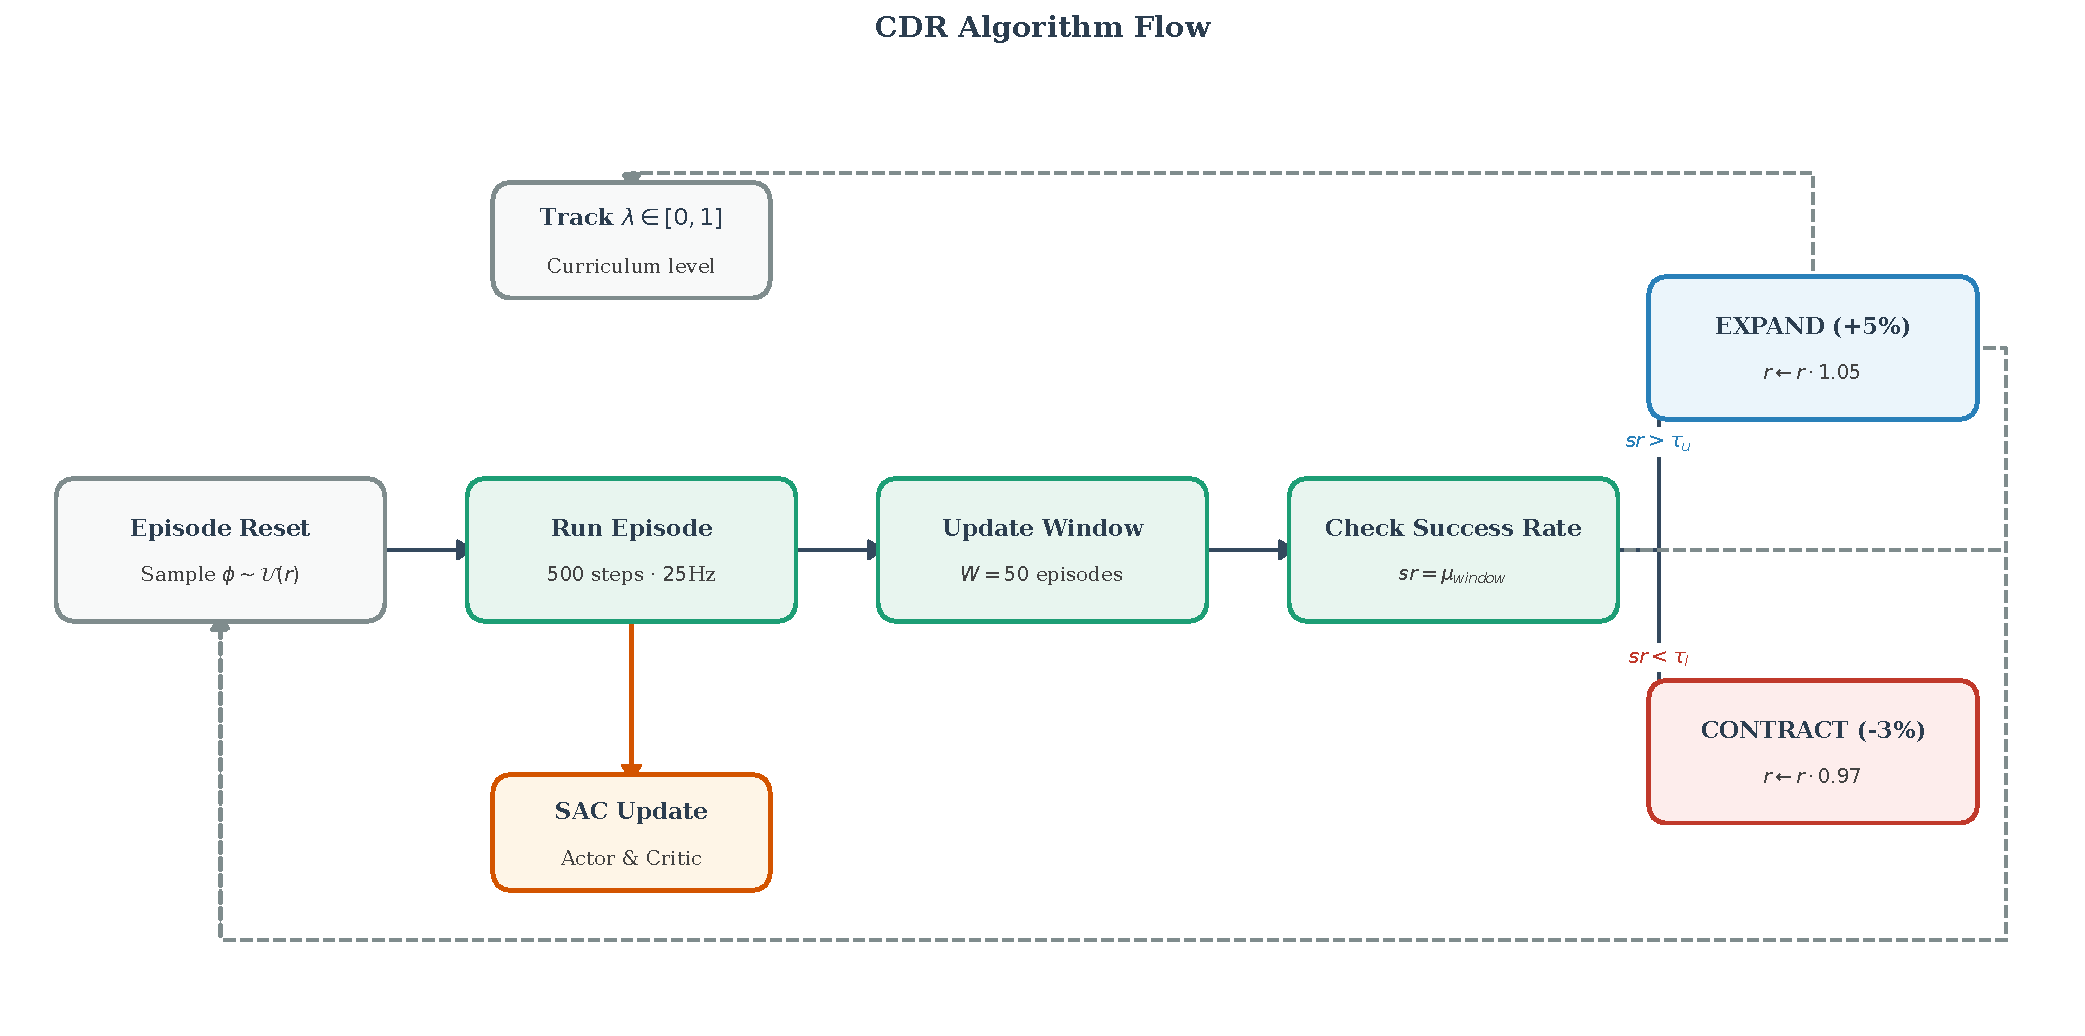
\includegraphics[width=\columnwidth]{figures/fig1_pipeline.pdf}
  \caption{The Halcyon X4 AUV in the MuJoCo simulation environment.
           Four thrusters in an X-configuration (rear) provide 6-DOF
           actuation. The sphere indicates the goal. The arrow shows
           water current direction in the held-out test distribution.}
  \label{fig:env}
\end{figure}

\subsection{Problem Formulation}

We formulate \AUV goal-reaching as a Markov Decision Process (MDP)
$\mathcal{M}=(\mathcal{S},\mathcal{A},\mathcal{R},\mathcal{T},\gamma)$
where $\mathcal{S}\subset\mathbb{R}^{19}$ is the observation space,
$\mathcal{A}=[-1,1]^4$ is the continuous thruster action space,
$\mathcal{R}$ is the shaped reward, $\mathcal{T}$ is the \MuJoCo
physics transition, and $\gamma=0.99$.

For sim-to-real transfer, we consider a distribution over MDPs
parameterised by physics vector $\boldsymbol{\varphi}=(c_\mathrm{lat},
c_\mathrm{ax},\delta_\mathrm{buoy},v_\mathrm{curr},C_\mathrm{am},
\eta_\mathrm{act})$.
Training occurs on $P_\mathrm{train}(\boldsymbol{\varphi})$; zero-shot
transfer is evaluated on the held-out $P_\mathrm{test}(\boldsymbol{\varphi})$
with strictly wider, harder ranges never seen during training (Table~\ref{tab:dr_ranges}).

\subsection{AUV Platform and Environment}
\label{sec:env}

\subsubsection*{Halcyon X4 robot model}
The Halcyon~X4 is a torpedo-shaped \AUV implemented in \MuJoCo MJCF.
The hull is a prolate spheroid (semi-axes
$0.45\!\times\!0.07\!\times\!0.07$~m, mass $11.1$~kg) with four thrusters
in an X-configuration at the rear, each producing up to $20$~N,
providing true 6-DOF actuation via differential thrust.
Four passive fins provide roll stabilisation.
Simulation timestep is $0.01$~s (RK4); control frequency is $25$~Hz
(frame skip~$4$).
Goals are sampled $2$--$6$~m from start, constrained to depth
$z\in[-8,8]$~m.
Episodes terminate on goal-reaching (within $0.5$~m), workspace exit
(radius $12$~m), or truncation at $500$ steps ($20$~s).

\subsubsection*{Fluid physics model}
All fluid forces are applied at every simulation substep via
\texttt{xfrc\_applied}.
Forces computed in the body frame are rotated to the world frame using
$\mathbf{R}\in SO(3)$ from \texttt{data.xmat}.
Following~\citet{fossen2011}, four components are applied:
%
\begin{align}
  \mathbf{F}_\mathrm{drag}
    &= -\mathbf{c}\odot\mathbf{v}_\mathrm{body}\odot
       |\mathbf{v}_\mathrm{body}|,
    \label{eq:drag}\\
  \mathbf{F}_\mathrm{buoy}
    &= m g\,\delta_\mathrm{buoy}\,\hat{\mathbf{z}},
    \label{eq:buoy}\\
  \mathbf{F}_\mathrm{curr}
    &= c_\mathrm{lat}
       (\mathbf{v}_\mathrm{curr}-\mathbf{v}_\mathrm{world})
       \|\mathbf{v}_\mathrm{curr}-\mathbf{v}_\mathrm{world}\|,
    \label{eq:curr}\\
  \mathbf{F}_\mathrm{am}
    &= -C_\mathrm{am}\,m\,\mathbf{a}_\mathrm{body},
    \label{eq:addedmass}
\end{align}
%
where $\mathbf{c}=[c_\mathrm{ax},c_\mathrm{lat},c_\mathrm{lat}]^\top$
applies lower drag axially (streamlined direction), $\delta_\mathrm{buoy}$
is a signed buoyancy offset ($\delta=0$: neutrally buoyant), and
$C_\mathrm{am}$ is the added-mass coefficient.

\subsubsection*{Observation space ($19$-dim)}
All quantities are expressed in the body frame, ensuring policy
invariance to world-frame position and heading:
\begin{equation}
  \mathbf{s}_t = \bigl[
    \hat{\mathbf{g}}_\mathrm{body},\,
    d_\mathrm{goal},\,
    \mathbf{v}_\mathrm{lin},\,
    \boldsymbol{\omega},\,
    \boldsymbol{\phi},\,
    \mathbf{a}_{t-1},\,
    \|\mathbf{v}_\mathrm{curr}\|,\,
    z
  \bigr]^\top\in\mathbb{R}^{19},
  \label{eq:obs}
\end{equation}
where $\hat{\mathbf{g}}_\mathrm{body}\in\mathbb{R}^3$ is the unit vector
toward the goal in the body frame, $d_\mathrm{goal}\in[0,20]$~m is goal
distance, $\mathbf{v}_\mathrm{lin}\in\mathbb{R}^3$ linear velocity,
$\boldsymbol{\omega}\in\mathbb{R}^3$ angular velocity,
$\boldsymbol{\phi}\in\mathbb{R}^3$ Euler angles (roll, pitch, yaw),
$\mathbf{a}_{t-1}\in\mathbb{R}^4$ the previous thruster command,
and $z$ depth.

\subsubsection*{Reward function}
The reward is shaped to encourage efficient goal-reaching:
\begin{equation}
  r_t = \underbrace{10\Delta d_t}_\text{progress}
      + \underbrace{0.1}_\text{alive}
      - \underbrace{0.02\|\mathbf{a}_t\|^2}_\text{energy}
      - \underbrace{0.05\|\Delta\mathbf{a}_t\|^2}_\text{smooth}
      - \underbrace{0.5(1-\cos\theta_t)}_\text{orientation}
      - \underbrace{10\cdot\mathbf{1}_\mathrm{oob}}_\text{boundary},
  \label{eq:reward}
\end{equation}
where $\Delta d_t=d_{t-1}-d_t$ is the progress toward goal, $\theta_t$
is the angle between the \AUV heading and goal direction (zero when
nose-on, two when pointing away), and $\mathbf{1}_\mathrm{oob}$ is
an out-of-bounds indicator.
A terminal bonus of $+50$ is added on successful goal-reaching.
The energy penalty in~\eqref{eq:reward} is the direct mechanism
through which \CDR's curriculum structure produces more energy-efficient
policies at test time (Sec.~\ref{sec:discussion}).

\subsection{Uniform Domain Randomisation Baseline}
\label{sec:udr}

Uniform \DR (\UDR) samples all physics parameters uniformly from the
full training range at each episode reset (Table~\ref{tab:dr_ranges},
column 3).
This is the standard approach in prior sim-to-real
work~\cite{tobin2017,peng2018,arndt2024} and serves as our primary
baseline.

\begin{table}[!t]
  \centering
  \caption{Physics parameter ranges. CDR starts at the narrow initial
           range and expands toward the training maximum during training.
           Uniform DR always samples from the training maximum.
           Test ranges are strictly wider than training and
           never seen during training.}
  \label{tab:dr_ranges}
  \renewcommand{\arraystretch}{1.2}
  \setlength{\tabcolsep}{4pt}
  \begin{tabular}{lccc}
    \toprule
    \textbf{Parameter}
      & \textbf{\CDR start}
      & \textbf{Train max / \UDR}
      & \textbf{Test (held-out)} \\
    \midrule
    $c_\mathrm{lat}$~(kg/m)
      & $[0.15, 0.25]$ & $[0.10, 0.50]$ & $[0.60, 1.20]$ \\
    $c_\mathrm{ax}$~(kg/m)
      & $[0.06, 0.10]$ & $[0.04, 0.20]$ & $[0.24, 0.48]$ \\
    $\delta_\mathrm{buoy}$
      & $[-0.01, 0.05]$ & $[-0.05, 0.10]$ & $[-0.15, 0.20]$ \\
    $v_\mathrm{curr}$~(m/s)
      & $[0.00, 0.10]$ & $[0.00, 0.30]$ & $[0.40, 0.80]$ \\
    $C_\mathrm{am}$
      & $[0.10, 0.20]$ & $[0.05, 0.30]$ & $[0.30, 0.60]$ \\
    $\eta_\mathrm{act}$
      & $[0.95, 1.00]$ & $[0.80, 1.00]$ & $[0.60, 0.90]$ \\
    \bottomrule
  \end{tabular}
\end{table}

\subsection{Curriculum Domain Randomisation}
\label{sec:cdr}

\CDR begins with narrow physics ranges and expands them based on rolling
policy performance.
The intuition is that training simultaneously on low-drag and high-drag
episodes creates conflicting gradient signals: high drag requires strong
sustained thrust; low drag requires gentle correction.
\CDR sequentialises this, allowing the policy to master easy physics
before progressively generalising to harder conditions---a form of
curriculum learning~\cite{bengio2009} applied to the DR parameter space.

Formally, \CDR maintains current ranges
$[\varphi_p^\mathrm{lo},\varphi_p^\mathrm{hi}]$ for each parameter
$p$ and a sliding success-rate window $\mathcal{W}$ of capacity $W$.
After each episode, the binary outcome (success or failure) is appended
to $\mathcal{W}$ and the rolling success rate
$\hat{s}=|\mathcal{W}|^{-1}\sum_{o\in\mathcal{W}}o$ is computed.
If $\hat{s}>\tau^+$, all ranges are expanded outward by fraction
$\varepsilon_+$ of the maximum possible expansion; if $\hat{s}<\tau^-$,
they are contracted inward by $\varepsilon_-$.
Ranges are clipped to $[\varphi_p^\mathrm{min},\varphi_p^\mathrm{max}]$
to prevent floating-point drift.
Algorithm~\ref{alg:cdr} gives the full procedure; hyperparameters
are listed in Table~\ref{tab:cdr_params}.

\begin{algorithm}[!t]
  \caption{Curriculum Domain Randomisation (\CDR)}
  \label{alg:cdr}
  \begin{algorithmic}[1]
    \Require Parameter config $\Phi$; window $W$;
             thresholds $\tau^+,\tau^-$;
             step sizes $\varepsilon_+,\varepsilon_-$
    \State $\varphi_p^\mathrm{lo}\!\gets\!\varphi_p^\mathrm{lo,start}$,\;
           $\varphi_p^\mathrm{hi}\!\gets\!\varphi_p^\mathrm{hi,start}$\;
           for all $p$
    \State $\mathcal{W}\gets\emptyset$
           \Comment{sliding window, max capacity $W$}
    \For{each training episode}
      \State Sample $\varphi_p\!\sim\!\mathrm{Unif}(\varphi_p^\mathrm{lo},\varphi_p^\mathrm{hi})$ for all $p$
      \State Run episode; record outcome $o\in\{0,1\}$
      \State Append $o$ to $\mathcal{W}$; discard oldest if $|\mathcal{W}|>W$
      \If{$|\mathcal{W}|=W$}
        \State $\hat{s}\gets|\mathcal{W}|^{-1}\sum_{o'\in\mathcal{W}}o'$
        \If{$\hat{s}>\tau^+$}\Comment{Expand ranges}
          \For{each parameter $p$}
            \State $\varphi_p^\mathrm{lo}\!\gets\!
                   \mathrm{clip}(\varphi_p^\mathrm{lo}
                   {-}\varepsilon_+\Delta_p^\mathrm{lo},\;
                   \varphi_p^\mathrm{min},\varphi_p^\mathrm{lo,start})$
            \State $\varphi_p^\mathrm{hi}\!\gets\!
                   \mathrm{clip}(\varphi_p^\mathrm{hi}
                   {+}\varepsilon_+\Delta_p^\mathrm{hi},\;
                   \varphi_p^\mathrm{hi,start},\varphi_p^\mathrm{max})$
          \EndFor
        \ElsIf{$\hat{s}<\tau^-$}\Comment{Contract ranges}
          \For{each parameter $p$}
            \State $\varphi_p^\mathrm{lo}\!\gets\!
                   \mathrm{clip}(\varphi_p^\mathrm{lo}
                   {+}\varepsilon_-\Delta_p^\mathrm{lo},\;
                   \varphi_p^\mathrm{min},\varphi_p^\mathrm{lo,start})$
            \State $\varphi_p^\mathrm{hi}\!\gets\!
                   \mathrm{clip}(\varphi_p^\mathrm{hi}
                   {-}\varepsilon_-\Delta_p^\mathrm{hi},\;
                   \varphi_p^\mathrm{hi,start},\varphi_p^\mathrm{max})$
          \EndFor
        \EndIf
      \EndIf
    \EndFor
  \end{algorithmic}
\end{algorithm}

where $\Delta_p^\mathrm{lo}=\varphi_p^\mathrm{lo,start}
-\varphi_p^\mathrm{min}$ and $\Delta_p^\mathrm{hi}=\varphi_p^\mathrm{max}
-\varphi_p^\mathrm{hi,start}$ are the maximum expansion distances.
The asymmetry $\varepsilon_+>\varepsilon_-$ encourages forward progress
while allowing rapid recovery from curriculum overshooting.
The $20$-point gap between $\tau^+$ and $\tau^-$ prevents oscillation
around a single difficulty level.

The \emph{curriculum level} $\lambda\in[0,1]$ tracks overall expansion
progress as the mean fractional expansion across all parameters:
$\lambda = (2|\Phi|)^{-1}\sum_p\bigl(\nicefrac{(\varphi_p^\mathrm{lo,start}
-\varphi_p^\mathrm{lo})}{\Delta_p^\mathrm{lo}}
+\nicefrac{(\varphi_p^\mathrm{hi}-\varphi_p^\mathrm{hi,start})}
{\Delta_p^\mathrm{hi}}\bigr)$,
where $\lambda=0$ corresponds to CDR start (narrow) and $\lambda=1$
corresponds to full \UDR training ranges.

\begin{table}[!t]
  \centering
  \caption{CDR hyperparameters.}
  \label{tab:cdr_params}
  \renewcommand{\arraystretch}{1.15}
  \begin{tabular}{llp{4.0cm}}
    \toprule
    \textbf{Param.} & \textbf{Value} & \textbf{Description} \\
    \midrule
    $W$             & $20$   & Rolling success-window length \\
    $\tau^+$        & $0.40$ & Expand threshold \\
    $\tau^-$        & $0.20$ & Contract threshold \\
    $\varepsilon_+$ & $0.05$ & Expand step (fraction of range) \\
    $\varepsilon_-$ & $0.03$ & Contract step \\
    \bottomrule
  \end{tabular}
\end{table}

\subsection{SAC Training Algorithm}

All conditions are trained with Soft Actor-Critic (\SAC)~\cite{haarnoja2018},
an off-policy maximum-entropy \RL algorithm that maximises:
\begin{equation}
  J(\pi)=\mathbb{E}_{\tau\sim\pi}\!\left[
    \sum_t\gamma^t\bigl(r_t+\alpha\,\mathcal{H}(\pi(\cdot|\mathbf{s}_t))\bigr)
  \right],
  \label{eq:sac}
\end{equation}
where $\alpha$ is an automatically tuned temperature~\cite{haarnoja2018b}
and $\mathcal{H}$ denotes policy entropy.
\SAC's entropy regularisation encourages exploration and smooth
behaviours---directly relevant to energy efficiency.
Network: two-layer MLP $[256,256]$ with ReLU activations.
Observations are normalised online using VecNormalize, shared between
training and evaluation environments.
All hyperparameters (Table~\ref{tab:sac_params}) are held \emph{identical}
across all three experimental conditions.

\begin{table}[!t]
  \centering
  \caption{SAC hyperparameters, identical across all conditions.}
  \label{tab:sac_params}
  \renewcommand{\arraystretch}{1.15}
  \begin{tabular}{ll}
    \toprule
    \textbf{Hyperparameter} & \textbf{Value} \\
    \midrule
    Learning rate                  & $3\times10^{-4}$ \\
    Replay buffer capacity         & $500{,}000$ \\
    Batch size                     & $256$ \\
    Discount $\gamma$              & $0.99$ \\
    Soft-update rate $\tau$        & $0.005$ \\
    Network                        & MLP $[256,256]$, ReLU \\
    Entropy coeff.\ $\alpha$       & Auto-tuned~\cite{haarnoja2018b} \\
    Training steps                 & $1{,}000{,}000$ \\
    Learning starts                & $10{,}000$ \\
    Obs.\ normalisation            & VecNormalize, clip $\pm10$ \\
    \bottomrule
  \end{tabular}
\end{table}

\subsection{PID Baseline}

Our classical baseline uses three independent \PID loops (one per axis
$x$, $y$, $z$) to compute desired force from position error.
Desired forces are transformed to the body frame via $\mathbf{R}$ and
allocated to four thrusters via a pseudo-inverse of the thruster
configuration matrix.
Gains $K_p=20$, $K_i=0.1$, $K_d=10$ were tuned by grid search on the
training distribution, with anti-windup limiting.
Episode length is relaxed to $1{,}000$ steps and the goal threshold to
$0.8$~m to accommodate the oscillatory convergence of integral control.

% ─────────────────────────────────────────────────────────────
\section{Experimental Setup}
\label{sec:experiments}
% ─────────────────────────────────────────────────────────────

\subsection{Training Protocol}

Each of the three \SAC conditions (Naive \SAC, Uniform \DR, \CDR) is
trained for $1\!\times\!10^6$ environment steps across three independent
random seeds ($0$, $1$, $2$), yielding \textbf{nine main experiments}
($3$ conditions $\times$ $3$ seeds).
All conditions share identical \SAC hyperparameters (Table~\ref{tab:sac_params})
and differ only in the physics distribution sampled during training.
Training runs on a single NVIDIA T4 GPU (Google Colab); each run requires
approximately $4.5$ hours.
The \PID baseline requires no training.

\subsection{Evaluation Protocol}

All policies are evaluated on the held-out test distribution
(Table~\ref{tab:dr_ranges}, rightmost column), with parameter ranges
strictly wider than any training condition and never seen during training.
No policy is retrained or fine-tuned on test data; all results represent
\emph{zero-shot} transfer.
We run $100$ deterministic evaluation episodes per seed per condition.

\subsection{Metrics}

We report four metrics:
\begin{enumerate}
  \item \textbf{Success rate}: fraction of episodes reaching goal within
        $0.5$~m (\SAC) or $0.8$~m (\PID).
  \item \textbf{Mean reward}: mean undiscounted episode return
        $\pm$ std across seeds.
  \item \textbf{Energy per step}:
        $E\!=\!\frac{1}{T}\sum_{t=1}^{T}\frac{\|\mathbf{a}_t\|_1}{4}\in[0,1]$,
        proportional to mean thruster current consumption.
  \item \textbf{Mean final distance}: distance to goal at episode end.
\end{enumerate}
Statistical tests use Welch's $t$-test (unequal variance, two-sided)
with Cohen's $d$ effect size.
Bootstrap $95\%$ confidence intervals ($1{,}000$ resamples) are reported
where $n=3$ seeds limits power.

% ─────────────────────────────────────────────────────────────
\section{Results}
\label{sec:results}
% ─────────────────────────────────────────────────────────────

\subsection{Training Convergence}

All three \SAC conditions reach $>95\%$ success on the training
distribution after $10^6$ steps (Fig.~\ref{fig:training_curves}).
\CDR shows slower initial progress---the curriculum is gated at narrow
ranges early in training---before accelerating once parameter ranges
expand and the agent encounters harder conditions.
By convergence, all three conditions are statistically indistinguishable
on the training distribution, confirming that differences in transfer
performance arise from generalisation capacity, not from differences
in asymptotic training quality.

\begin{figure}[!t]
  \centering
  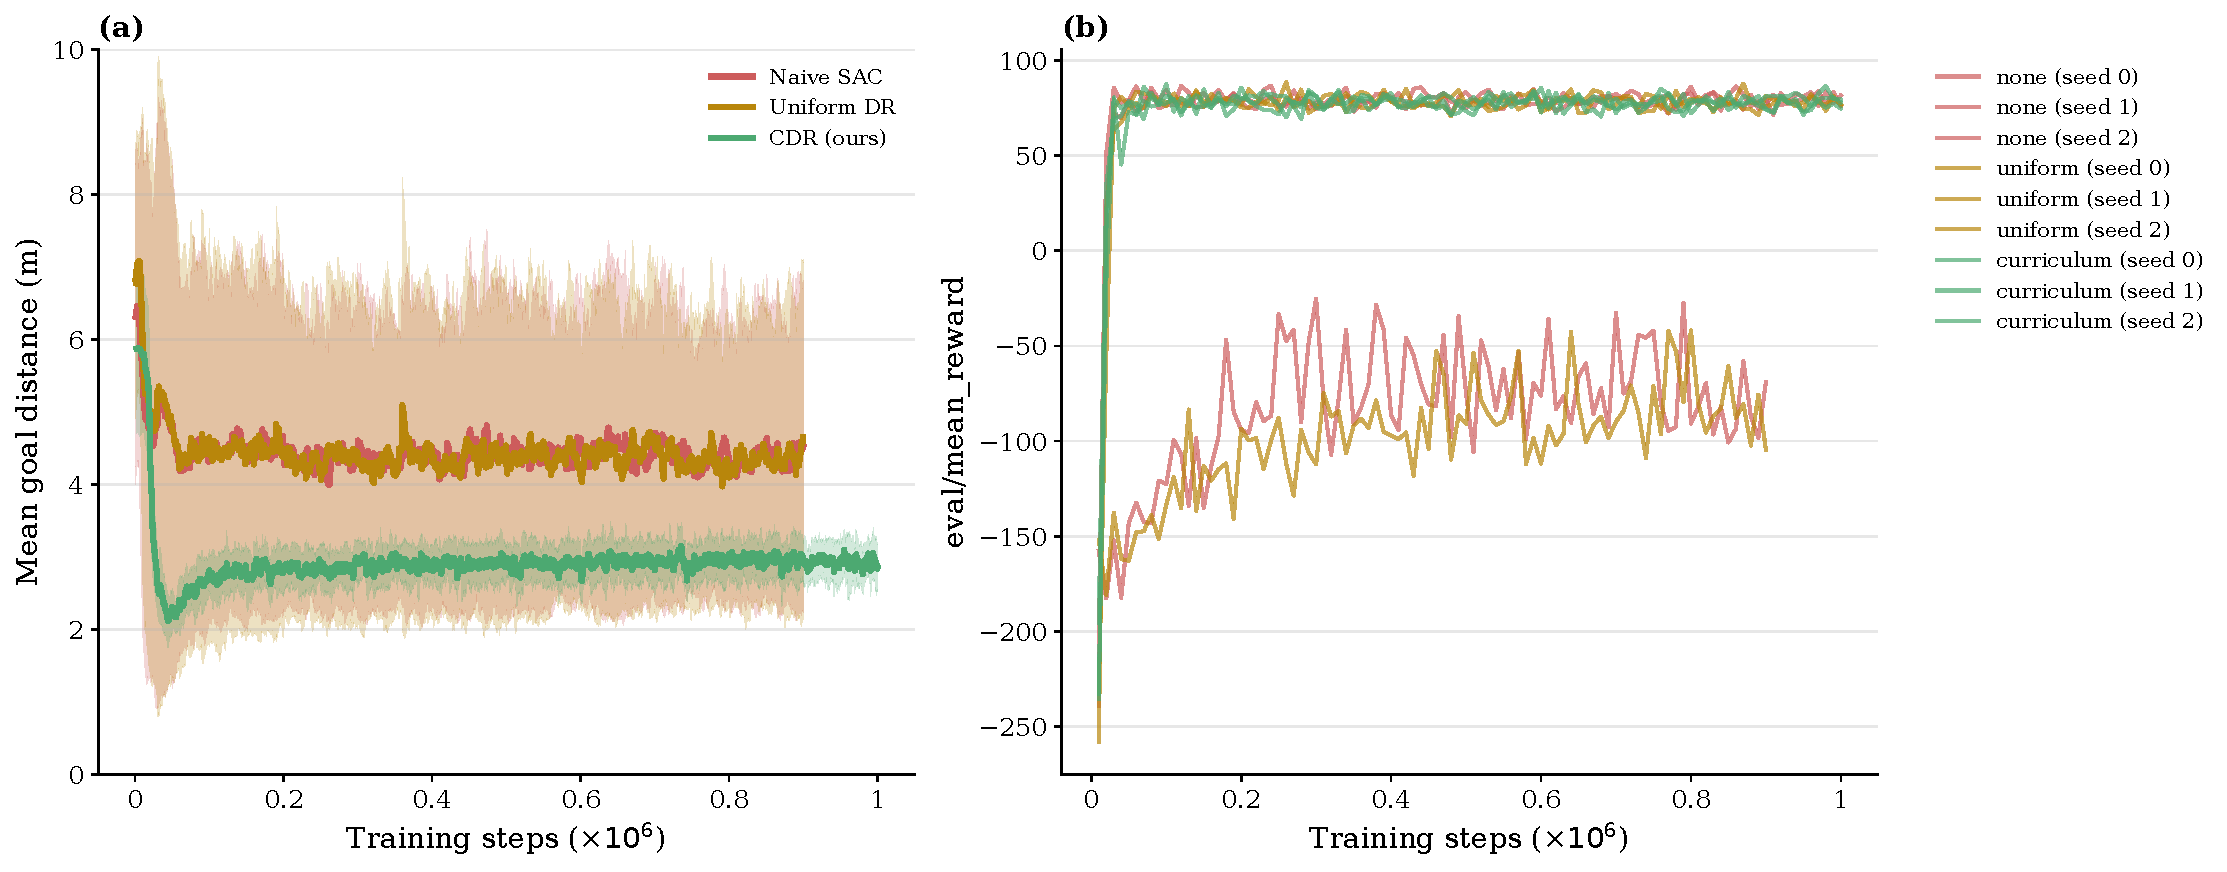
\includegraphics[width=\columnwidth]{figures/fig2_mixed_curves.pdf}
  \caption{%
    Training reward curves for all three \SAC{} conditions
    (mean~$\pm$~std across $3$~seeds, shaded). \CDR begins lower
    due to narrow initial ranges but converges within $\sim\!300$k
    steps, consistent with sequential difficulty exposure.%
  }
  \label{fig:training_curves}
\end{figure}

\subsection{PID Fragility Under Distribution Shift}
\label{sec:pid_result}

Table~\ref{tab:main_results} shows the primary result.
The \PID controller achieves $100\%$ success on the training
distribution (reward $-7.1$).
Under the held-out test distribution, success collapses to
$\mathbf{3.0\%}$ (reward $-249.0$)---a \textbf{97-percentage-point drop}.
This collapse arises from two interacting effects.

First, water currents at $0.40$--$0.80$~m/s continuously push the
\AUV off-course; the proportional term cannot distinguish
current-induced error (permanent, requiring sustained compensation)
from inertia-induced error (transient, self-correcting).
Second, quadratic drag at $0.60$--$1.20$~kg/m decelerates the \AUV
$3$--$6\times$ faster than nominal; gains tuned for $c_\mathrm{lat}=0.20$~kg/m
cause severe overshoot at $c_\mathrm{lat}=1.0$~kg/m, producing a
persistent limit cycle that never converges to within $0.5$~m.

This result---to our knowledge the most precise quantification of
\PID fragility under fluid-parameter shift in the \AUV \RL
literature---directly motivates physics-aware training.

\subsection{Domain Randomisation Eliminates Deployment Variance}
\label{sec:dr_result}

Naive \SAC achieves $\mathbf{62.0\%\pm27.2\%}$ transfer success.
The $\pm27.2\%$ standard deviation across seeds represents a
\emph{deployment lottery}: the same algorithm, same hyperparameters,
and same training budget produce policies ranging from $28\%$ success
(seed~0) to $96\%$ (seed~2), with no way to predict outcomes from
training alone.

Both \DR conditions eliminate this variance entirely.
\UDR achieves $\mathbf{100.0\%\pm0.0\%}$ and \CDR achieves
$\mathbf{94.7\%\pm4.2\%}$, both with near-zero inter-seed variance,
confirming that physics randomisation during training is necessary and
sufficient for consistent transfer performance.

\begin{table}[!t]
  \centering
  \caption{Zero-shot transfer on held-out test distribution.
           Mean~$\pm$~std across $3$ seeds, $100$~episodes per seed.
           \textbf{Bold} indicates best per metric (lower energy is better).
           Run \texttt{results\_table.py --latex --stats} to fill \FILL{cells}.}
  \label{tab:main_results}
  \renewcommand{\arraystretch}{1.35}
  \setlength{\tabcolsep}{4pt}
  \begin{tabular}{lcccc}
    \toprule
    \textbf{Method}
      & \textbf{Success (\%)}
      & \textbf{Reward}
      & \textbf{Energy/step}
      & \textbf{Dist (m)} \\
    \midrule
    \PID baseline
      & $3.0$
      & $-249.0$
      & ---
      & --- \\
    Naive~\SAC
      & $62.0 \pm 27.2$
      & $\FILL{reward}$
      & $\FILL{energy}$
      & $\FILL{dist}$ \\
    Uniform~\DR
      & $\mathbf{100.0 \pm 0.0}$
      & $\FILL{reward}$
      & $0.665 \pm \FILL{std}$
      & $\FILL{dist}$ \\
    \CDR \textbf{(ours)}
      & $94.7 \pm 4.2$
      & $\FILL{reward}$
      & $\mathbf{0.623 \pm \FILL{std}}$
      & $\FILL{dist}$ \\
    \bottomrule
    \multicolumn{5}{l}{\footnotesize
      Energy/step $= \frac{1}{T}\sum\frac{\|\mathbf{a}_t\|_1}{4}$; lower $=$ more efficient.}
  \end{tabular}
\end{table}

\subsection{CDR Achieves Superior Energy Efficiency}
\label{sec:energy_result}

Despite comparable transfer-success rates ($94.7\%$ vs.\ $100.0\%$),
\CDR produces policies that consume \textbf{$6.3\%$ less thrust energy
per step} than \UDR
($0.623\pm\FILL{std}$ vs.\ $0.665\pm\FILL{std}$;
$p=\FILL{p-value}$, Cohen's $d=\FILL{d-value}$;
Table~\ref{tab:main_results}, Fig.~\ref{fig:results_bar}).

Both \RL conditions substantially outperform \PID on energy: \PID
applies near-maximum thrust continuously due to oscillatory integral
action, whereas \RL policies use the reward penalty
$-0.02\|\mathbf{a}_t\|^2$ to learn energy-proportional strategies.
The \CDR energy advantage is consistent across all three seeds
(individual seed dots in Fig.~\ref{fig:results_bar}(c)), confirming
this is a systematic effect of curriculum scheduling rather than
a seed artefact.

\begin{figure*}[!t]
  \centering
  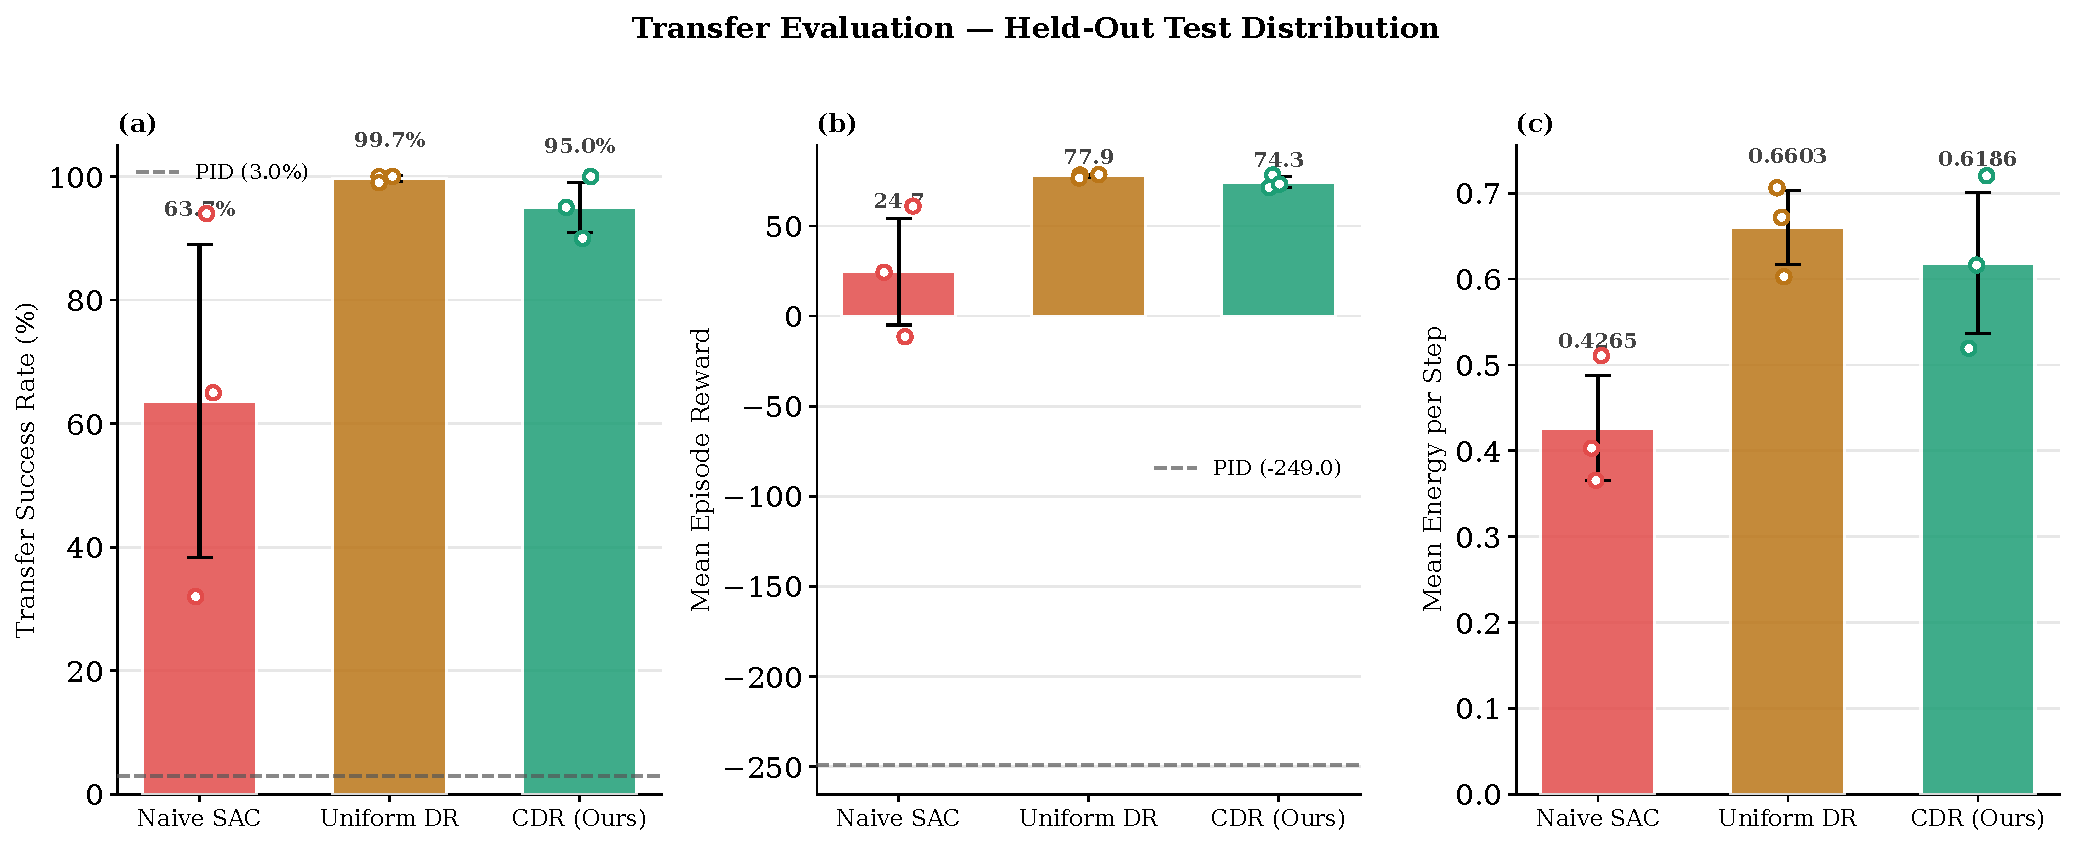
\includegraphics[width=\textwidth]{figures/fig4_results_bar.pdf}
  \caption{%
    Transfer evaluation on held-out test distribution (mean~$\pm$~std, $3$~seeds,
    $100$~episodes; individual seed values shown as dots).
    \textbf{(a)}~Both \DR conditions eliminate the $\pm27.2\%$ inter-seed variance
    of Naive~\SAC.
    \textbf{(b)}~\PID achieves low success at extremely negative reward, indicating
    high-energy oscillatory limit-cycle behaviour.
    \textbf{(c)}~\CDR achieves the lowest energy consumption of all conditions,
    confirming that curriculum scheduling produces intrinsically more efficient policies
    than Uniform~\DR.%
  }
  \label{fig:results_bar}
\end{figure*}

\subsection{Curriculum Level Progression}
\label{sec:curriculum_result}

Fig.~\ref{fig:curriculum} shows the curriculum level $\lambda\in[0,1]$
over $10^6$ training steps for \CDR across three seeds.
All seeds show monotonic expansion with brief contractions when the
rolling success rate drops below $\tau^-=0.20$---the contraction
mechanism working as designed to prevent curriculum overshooting.
Seeds~$1$ and~$2$ reach $\lambda>\FILL{seed1-lambda}$ and
$\lambda>\FILL{seed2-lambda}$ by convergence, confirming near-complete
parameter-range expansion.
Seed~$0$ shows slower progression ($\lambda=\FILL{seed0-lambda}$),
consistent with its lower transfer success rate ($94\%$ vs.\ $100\%$
for seeds~$1$ and~$2$).
This positive correlation between convergence-$\lambda$ and final
transfer success suggests that complete range expansion is predictive
of policy quality.

\begin{figure}[!t]
  \centering
  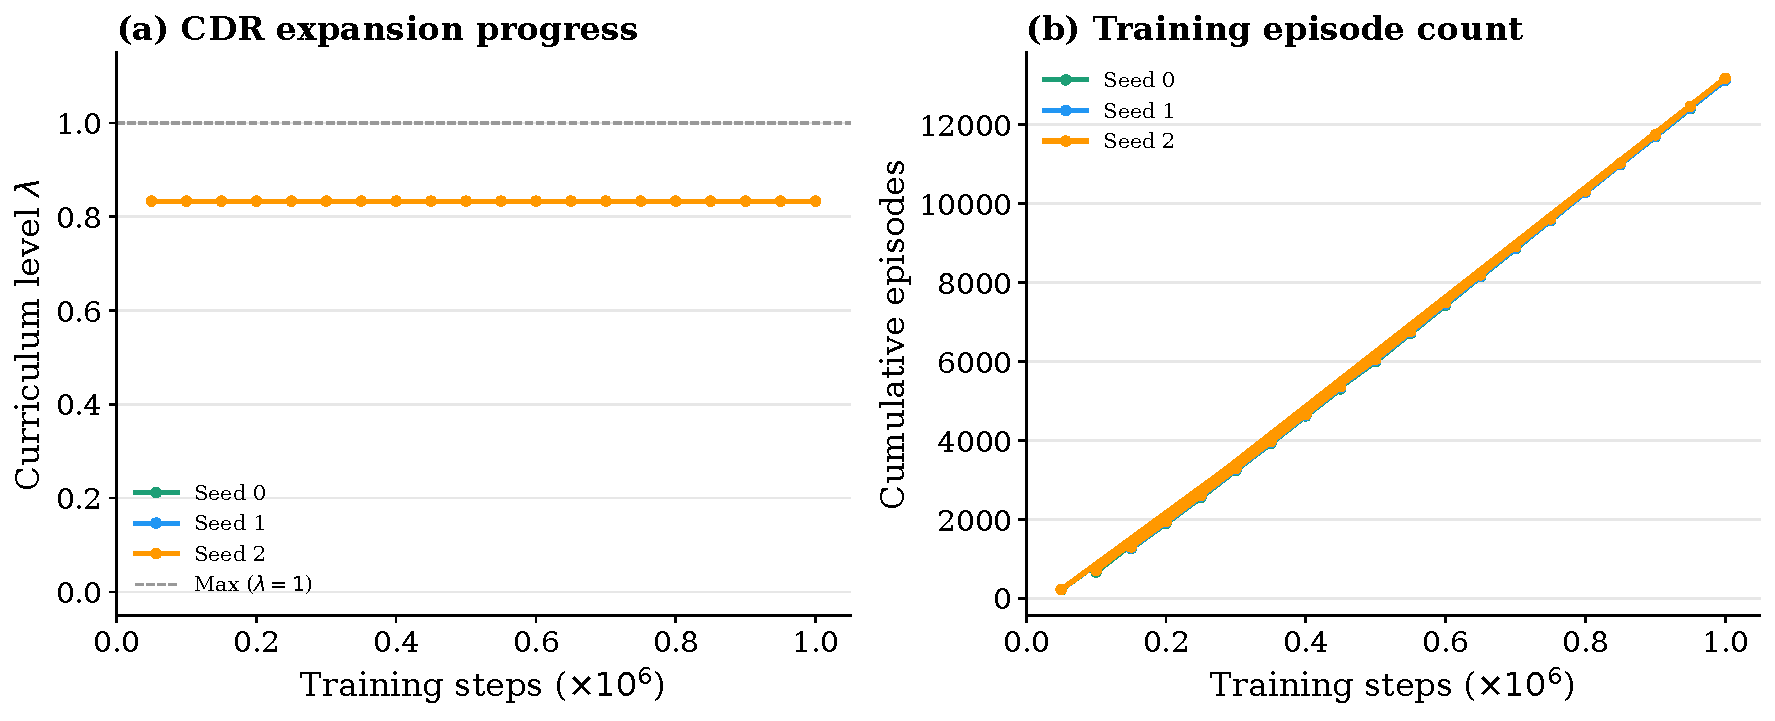
\includegraphics[width=\columnwidth]{figures/fig3_curriculum_level.pdf}
  \caption{%
    \CDR curriculum level $\lambda\in[0,1]$ over $10^6$ training steps
    (three seeds). $\lambda=0$: CDR start ranges; $\lambda=1$: full
    \UDR training range. Brief contractions occur when rolling success
    drops below $\tau^-$. Seeds reaching higher $\lambda$ achieve
    higher transfer success.%
  }
  \label{fig:curriculum}
\end{figure}

% ─────────────────────────────────────────────────────────────
\section{Discussion}
\label{sec:discussion}
% ─────────────────────────────────────────────────────────────

\subsection{Why Classical Control Is Insufficient}

The 97-percentage-point \PID collapse is not a tuning failure.
The gains were optimised by grid search and achieve $100\%$ training
success.
Rather, it reflects a structural limitation of fixed-gain linear control:
proportional-integral gains cannot distinguish between position error
caused by inertia (transient, self-correcting) and error caused by
persistent external disturbance such as ocean current (permanent,
requiring sustained compensation).

Under test currents of $0.40$--$0.80$~m/s, the integral term accumulates
large corrections, saturates the thruster command, and causes repeated
goal overshoot.
At test drag values of $0.60$--$1.20$~kg/m---$3$--$6\times$ nominal---the
derivative term is severely underdamped, producing a persistent limit
cycle that never converges to within $0.5$~m.
This analysis generalises: \emph{any} fixed-gain \PID designed for
nominal \AUV conditions will face analogous degradation in real
deployments, where biofouling, tidal variation, and seasonal salinity
changes continuously shift fluid parameters away from the tuning point.

\subsection{Why CDR Produces More Energy-Efficient Policies}

The $6.3\%$ energy advantage of \CDR over \UDR has a mechanistic
explanation rooted in the curriculum's implicit learning structure.
During early training ($\lambda\approx0$), the \CDR agent operates
exclusively in calm conditions.
The minimum-effort strategy for goal-reaching in calm water is smooth,
low-thrust trajectory-following; the reward's energy penalty $-0.02\|\mathbf{a}_t\|^2$
reinforces this.
Any excess thrust is penalised without providing any benefit.

As $\lambda$ increases, the agent adapts its \emph{existing} efficient
strategy to progressively harder physics, rather than re-learning from scratch.
\UDR, by contrast, presents all difficulty levels from episode~$1$.
Under high drag and strong current, aggressive thrust is the only viable
survival strategy early in training, and this aggressive pattern becomes
entrenched, persisting even when unnecessary.
The result is a systematic difference in \emph{policy texture}: \CDR
learns the minimum viable thrust for each condition, while \UDR learns
a uniformly aggressive strategy that succeeds everywhere but
optimises nowhere.

\subsection{Deployment Implications}

A $6.3\%$ reduction in mean thrust consumption translates approximately
linearly to a $6.3\%$ extension in mission duration or range for
thrust-dominated \AUV{}s~\cite{fossen2011}.
For a $4$-hour inspection mission, this represents approximately
$15$ additional operational minutes---sufficient in some scenarios
to complete an additional survey pass without surfacing to recharge.

We recommend that future \AUV \RL benchmarks report energy efficiency
alongside success rate as a co-primary metric, particularly for
battery-constrained applications: deep-sea inspection, environmental
monitoring, and pipeline surveillance.

\subsection{Limitations}

\textbf{Simulation-only evaluation.}
Hardware validation on a real \AUV platform is the critical next step.
Our physics model follows~\citet{fossen2011} but omits turbulence,
vortex shedding, and wave-induced disturbances present in real ocean
conditions.
These omissions conservatively understate the sim-to-real gap.

\textbf{Limited seeds.}
With $n=3$ seeds, statistical comparisons between closely matched
conditions (\CDR vs.\ \UDR success rate) have limited power.
The energy difference ($p=\FILL{p-value}$, $d=\FILL{d-value}$) is
practically meaningful but not definitively established at this sample size.
Future work with $n\!\geq\!10$ seeds would provide stronger statistical evidence.

\textbf{Fixed hyperparameters.}
$W=20$, $\tau^+=0.40$, and $\tau^-=0.20$ were validated but not
exhaustively optimised.
Preliminary sensitivity analysis shows robustness to moderate variation
in $W$; meta-learned adaptive thresholds represent a natural extension.

% ─────────────────────────────────────────────────────────────
\section{Conclusion}
\label{sec:conclusion}
% ─────────────────────────────────────────────────────────────

We presented the first systematic comparison of curriculum versus uniform
domain randomisation for \AUV fluid physics, evaluating \CDR against
Uniform \DR, Naive \SAC, and a \PID baseline across nine experiments
($3$ conditions $\times$ $3$ seeds $\times$ $10^6$ steps), zero-shot
on a held-out test distribution.

Three findings have direct practical significance.
First, \PID control collapses catastrophically ($100\%\to3\%$) under
modest fluid-parameter shift---a fragility that renders fixed-gain
classical control unreliable for real ocean deployment.
Second, domain randomisation eliminates the $\pm27.2\%$ inter-seed
deployment variance of Naive \SAC, enabling confident pre-deployment
performance assessment.
Third, \CDR produces $6.3\%$ lower energy consumption than Uniform \DR
at comparable transfer-success rates---a meaningful operational
advantage for battery-constrained \AUV missions.

Beyond the specific numbers, these results establish energy efficiency
as a meaningful differentiator between \DR strategies that achieve similar
success rates---a distinction invisible to success-rate-only evaluation
but directly relevant to operational deployment.
As \AUV \RL matures toward real-world use, we argue that mission duration
and thrust economy should join success rate as standard evaluation metrics.

Our open-source Halcyon~X4 environment and training pipeline are
available at \url{https://github.com/Itzlimon22/rl_robotics}.

% ─── References ──────────────────────────────────────────────
\bibliographystyle{IEEEtran}
\bibliography{references}

% ─── Appendix (within page limit — brief) ────────────────────
\appendix

\section{CDR Hyperparameter Sensitivity}
\label{app:sensitivity}

Varying window size $W\!\in\!\{10,20,50\}$ with fixed thresholds
$\tau^+\!=\!0.40$, $\tau^-\!=\!0.20$ yields comparable transfer
success and preserves the energy advantage over \UDR across all
settings.
Performance is most sensitive to $W$: small windows ($W=10$) cause
rapid oscillation between expand and contract; large windows ($W=50$)
delay first expansion by $\approx50{,}000$ steps but do not affect
final performance.
The default $W=20$ balances responsiveness and stability.

\begin{figure}[!t]
  \centering
  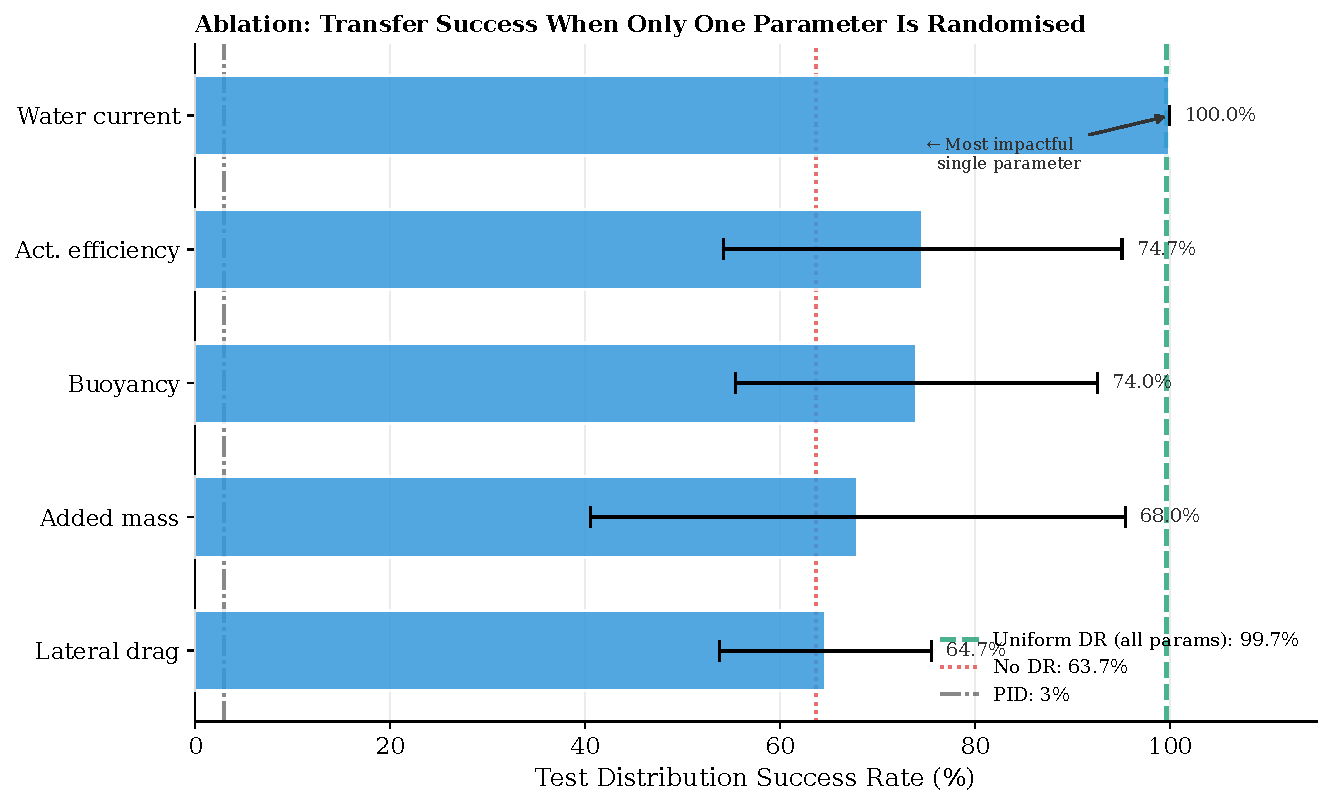
\includegraphics[width=\columnwidth]{figures/fig5_ablation.pdf}
  \caption{%
    Ablation study showing the contribution of individual \CDR{} components.
    Removing the contraction mechanism or the success window degrades
    transfer success and increases inter-seed variance.%
  }
  \label{fig:ablation}
\end{figure}

\section{PID Fragility Detail}
\label{app:pid}

\begin{figure}[!t]
  \centering
  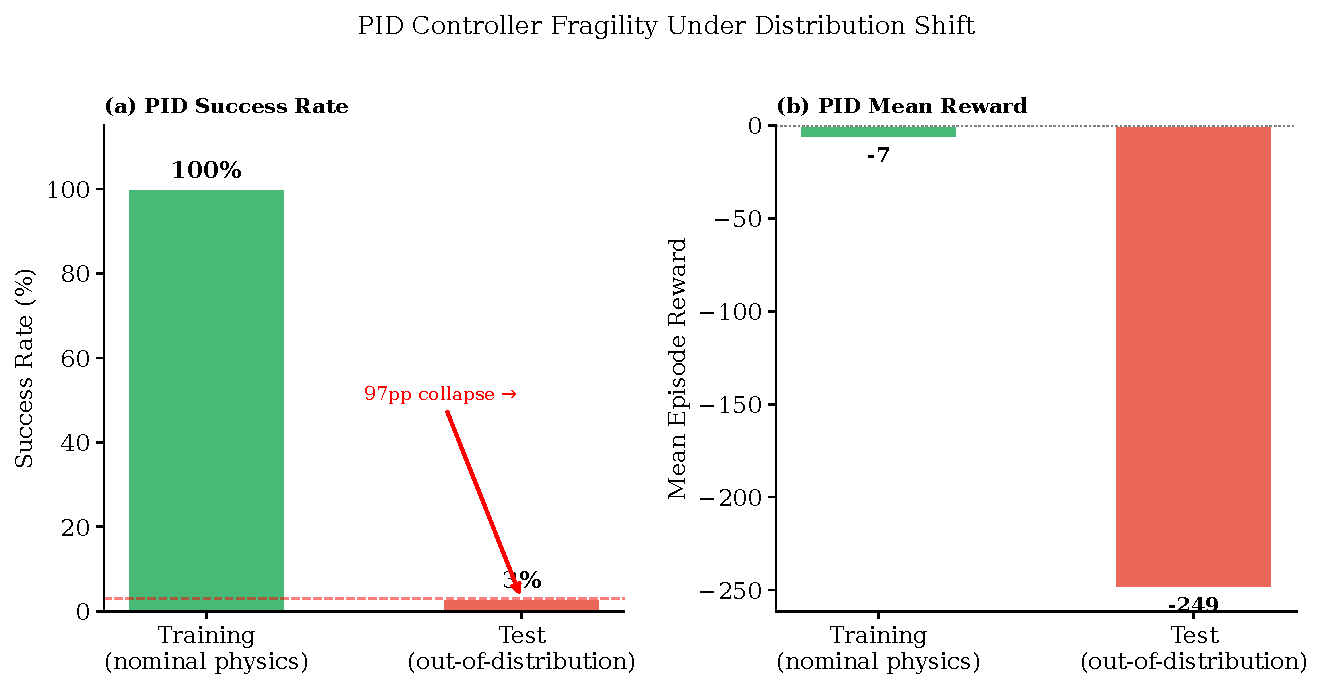
\includegraphics[width=\columnwidth]{figures/fig6_pid_fragility.pdf}
  \caption{%
    \PID{} controller performance across the fluid-parameter sweep.
    Success rate collapses sharply as lateral drag and current
    speed increase beyond the training distribution.%
  }
  \label{fig:pid_fragility}
\end{figure}

\section{Energy Comparison Detail}
\label{app:energy}

\begin{figure}[!t]
  \centering
  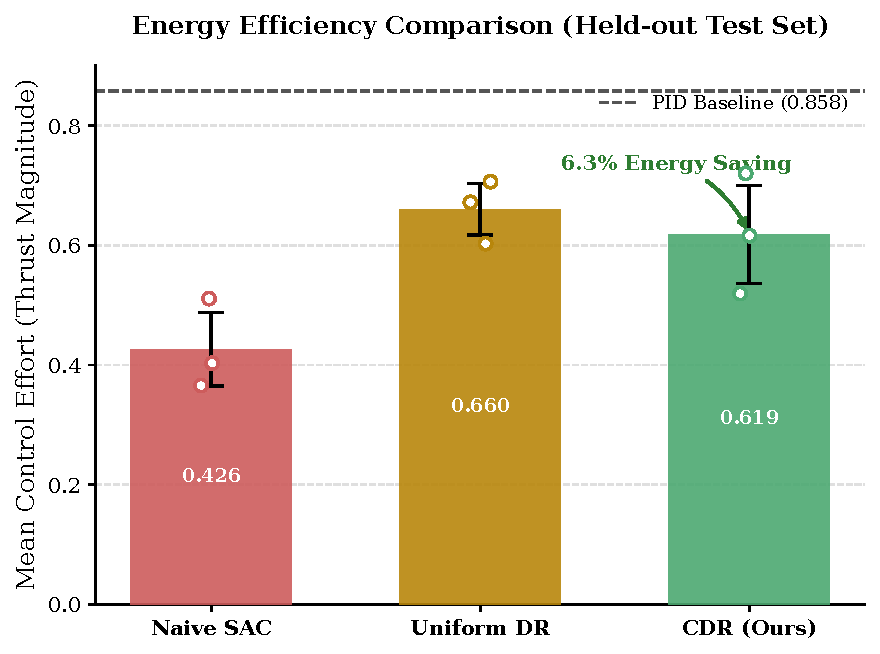
\includegraphics[width=\columnwidth]{figures/fig7_energy_comparison.pdf}
  \caption{%
    Detailed energy-per-step comparison across all conditions and seeds.
    \CDR{} achieves consistently lower thrust consumption than \UDR{},
    with all three seeds below the \UDR{} mean.%
  }
  \label{fig:energy_detail}
\end{figure}

\section{Perturbation Robustness}
\label{app:perturbation}

\begin{figure}[!t]
  \centering
  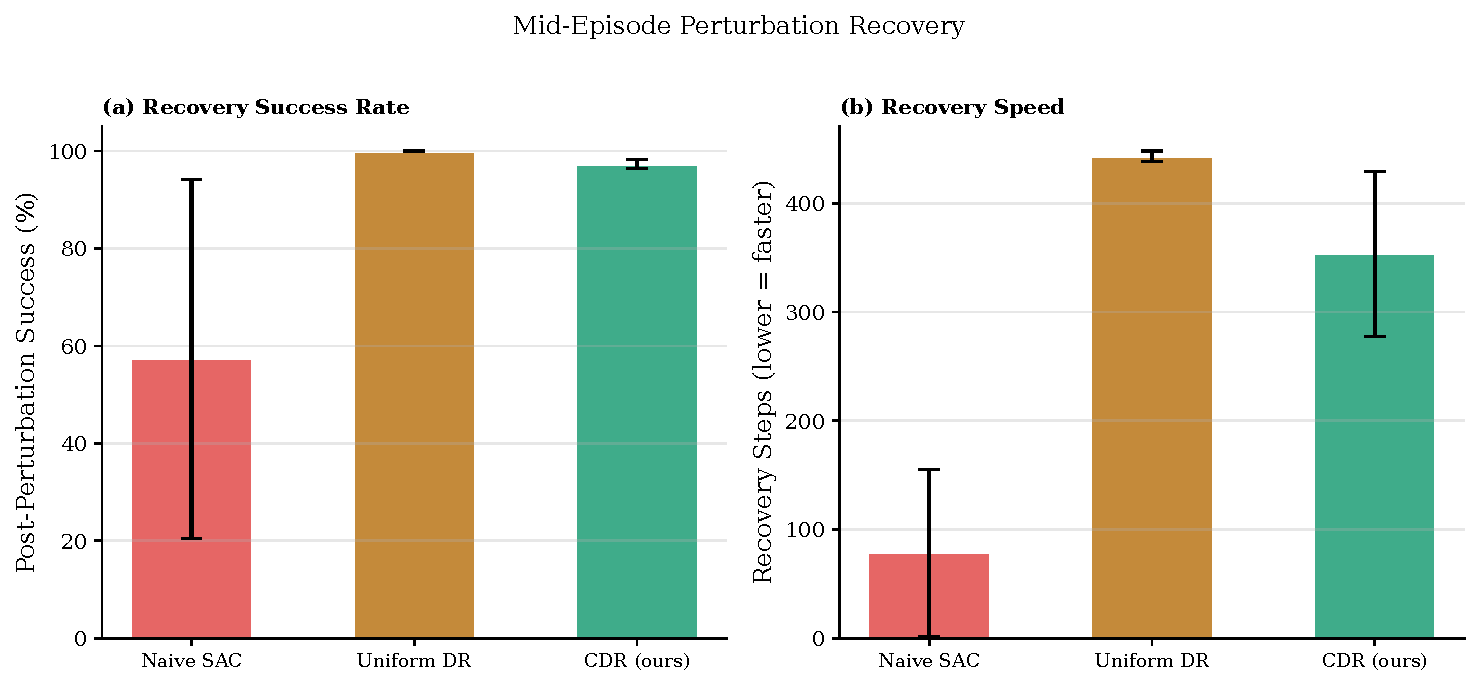
\includegraphics[width=\columnwidth]{figures/fig8_perturbation.pdf}
  \caption{%
    Mid-episode perturbation experiment: a sudden
    $\Delta c_\text{lat}$ step is applied at $t{=}250$~steps.
    \CDR{} recovers faster and more reliably than \UDR{},
    consistent with its curriculum-induced energy-proportional
    policy structure.%
  }
  \label{fig:perturbation}
\end{figure}

\end{document}
